%PDF DI RIFERIMENTO: 03_Requirement Engineering.pdf

\chapter{Requirement Analysis}
    \section{Obiettivo}
        In questa sezione verranno analizzate le informazioni definite nei requisiti di sistema al fine di schematizzare opportunamente il dominio del problema.

    \section{Use Case Diagram}
        %Use Case Diagram costruito con StarUML
        \begin{figure}[htbp!]
            \centering
                \vspace{2\baselineskip}
                \includegraphics[width=0.35\linewidth]{Immagini/Diagrammi/UseCaseDiagram.pdf}
            \caption{Use Case Diagram}
            \label{fig:Use Case Diagram}
        \end{figure}

    \newpage
    
    \section{Target utenti}
        La personas principale scelta è Maria Lombardo. La personas secondaria è Luca Serra
        
        \begin{figure}[!htb]
           \begin{minipage}{0.48\textwidth}
                \centering
             \includegraphics[width=.7\linewidth]{Immagini/Personas/Maria Lombardo.pdf}
             \caption{Maria Lombardo}\label{Fig:Maria Lombardo}
           \end{minipage}\hfill
           \begin{minipage}{0.48\textwidth}
                \centering
             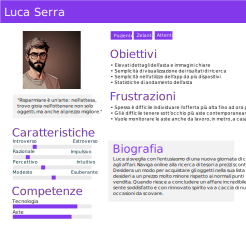
\includegraphics[width=.7\linewidth]{Immagini/Personas/Luca Serra.pdf}
             \caption{Luca Serra}\label{Fig:Luca Serra}
           \end{minipage}
        \end{figure}

        \begin{figure}[!htb]
           \begin{minipage}{0.48\textwidth}
                \centering
             \includegraphics[width=.7\linewidth]{Immagini/Personas/Marco Rossi.pdf}
             \caption{Marco Rossi}\label{Fig:Marco Rossi}
           \end{minipage}\hfill
           \begin{minipage}{0.48\textwidth}
                \centering
             \includegraphics[width=.7\linewidth]{Immagini/Personas/Martina Silvestri.pdf}
             \caption{Martina Silvestri}\label{Fig:Martina Silvestri}
           \end{minipage}
        \end{figure}

        \begin{figure}[!htb]
           \begin{minipage}{0.48\textwidth}
                \centering
             \includegraphics[width=.7\linewidth]{Immagini/Personas/Matteo Luongo.pdf}
             \caption{Matteo Luongo}\label{Fig:Matteo Luongo}
           \end{minipage}\hfill
           \begin{minipage}{0.48\textwidth}
                \centering
             \includegraphics[width=.7\linewidth]{Immagini/Personas/Arturo Campobello.pdf}
             \caption{Arturo Campobello}\label{Fig:Arturo Campobello}
           \end{minipage}
        \end{figure}
        
    \section{Mockup}

    \section{Tabelle di Cockburn}